\documentclass[12pt,fleqn]{article}\usepackage{../../common}
\begin{document}
Renk, Bölgeler ve Doku (Texture)

Renk Nicemlemesi, Posterleme (Color Quantization, Posterization)

Bir resimdeki en yaygın renkleri bulmak için [2],

\begin{minted}[fontsize=\footnotesize]{python}
from thief import ColorThief
color_thief = ColorThief('t00100.jpg')
colors = color_thief.get_palette(color_count=20)  
import matplotlib.colors as mcolors
colors = [np.array(x)/255. for x in colors]
my_cmap = mcolors.ListedColormap(colors)
plt.figure(figsize=(20, 0.5))
plt.pcolormesh(np.arange(my_cmap.N).reshape(1, -1), cmap=my_cmap)
plt.gca().yaxis.set_visible(False)
plt.gca().set_xlim(0, my_cmap.N)
plt.savefig('vision_50colreg_02.png')
\end{minted}


\includegraphics[width=15cm]{vision_50colreg_02.png}

Şimdi resmin yaygın renklerinden birinin (üstteki renklerde en sağdaki kırmızı
mesela) resmin hangi piksellerine en yakın olduğunu bulalım. Basit uzaklık
ölçüsü kullanarak H,S,V renk üçlüsü üzerinden bir uzaklık hesaplayacağız, belli
bir eşik değeri altında olan tüm pikselleri mavi ile göstereceğiz.

\begin{minted}[fontsize=\footnotesize]{python}
import colorsys, pandas as pd
from PIL import Image
A = np.array(Image.open('t00100.jpg').convert('HSV'))
A2 = A.reshape(640*360, 3)
idx = np.array([[j, i] for i in range(360) for j in range(640)])
df = pd.DataFrame(np.hstack((A2,idx)))
df.columns = ['c1','c2','c3','x','y']

colors2 = [x*255. for x in colors]
colors3 = [colorsys.rgb_to_hsv(x[0], x[1], x[2]) for x in colors2]

diff = (df[['c1','c2','c3']] - colors2[18]).abs().sum(axis=1)
df2 = df[diff < 100.]
A3 = np.array(Image.open('t00100.jpg'))
plt.imshow(A3)
plt.hold(True)
plt.plot(df2.x,df2.y,'.')
plt.savefig('vision_50colreg_01.png')
\end{minted}

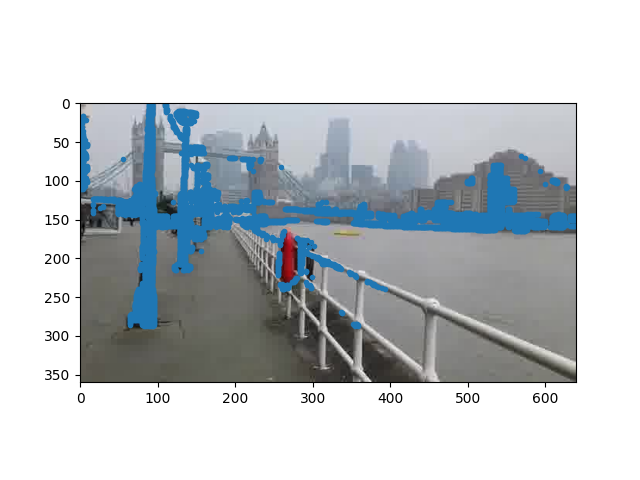
\includegraphics[width=15cm]{vision_50colreg_01.png}

Uzaklık için özellikle R,G,B değil H,S,V kullandık çünkü bu renk temsilinin
uzaklık hesaplarında daha iyi işlediği biliniyor. 

Bölgeler Eşit mi?

İki imaj bölgesinin birbiriyle aynı mı farklı mı olduğu sorusu imaj gruplaması
(segmentation) ya da kümelemesi için önemli bir soru. Elimizde iki piksel grubu
var, birinin diğerine ait olduğunu nasıl bileceğiz?

İlginç bir çözüm şu olabilir; piksel değerlerinin bir olasılık dağılımından
örneklendiğini düşünmek, ve her iki bölgenin aynı dağılımdan gelip gelmediğini
kontrol etmek [1, sf. 99].

Diyelim ki belli bir düzeni, yapısı olan bir imaj bölgesi aynı / sabit bir gri
değerinin, istatistiki olarak bağımsız, 0-değerli Gaussian'dan gelen bir gürültü
eklenmiş hali. Elimizde iki bölge var, $R_1,R_2$, içlerinde sırasıyla $m_1,m_2$
tane piksel değeri var. İki hipotez mümkün,

$H_0$: Her iki bölge aynı objeye ait. Bu durumda her iki bölgenin tüm gri renk
değerleri tek bir Gaussian'dan örneklenmiştir, ki bu Gaussian $(\mu_0,\sigma_0^2)$
olsun.

$H_1$: İmaj bölgeleri / pikselleri farklı objelere ait. Bu durumda her piksel
grubu ayrı Gaussian dağılımından geliyor, 1. bölge $(\mu_1,\sigma_1^2)$,
2. bölge $(\mu_2,\sigma_2^2)$.

Çoğunlukla bu parametreler bilinmez, maksimum olurluk (likelihood) kullanılarak
veriden kestirilirek hesaplanır,

$$ \hat{\mu} = \frac{1}{n} \sum _{i=1}^{n}g_i $$

$$ \hat{\sigma} = \frac{1}{n} \sum _{i=1}^{n} (g_i-\hat{\mu})^2 $$

Bunlar temel istatistikten bildiğimiz şeyler.  Simdi herhangi bir $\mu,\sigma$
için bir piksel değeri $g_i$'in olasılığı

$$ p(g_i) = \frac{1}{\sqrt{2\pi} \sigma_0} \exp (- (g_i-\mu_0)^2 / 2\sigma^2)  $$

$H_0$ altında tüm pikseller aynı dağılımdan geliyor, o zaman tüm verileri
gözönüne alan ortak dağılım,

$$ p(g_1,g_2,...,g_{m_1+m_2} | H_0) = \prod _{i=1}^{m_1+m_2} p(g_i|H_0)$$

$$
= \prod _{i=1}^{m_1+m_2} \frac{1}{\sqrt{2\pi} \sigma_0}
\exp (- (g_i-\mu_0)^2 / 2\sigma_0^2) )
$$

$$
= \frac{1}{ (\frac{1}{\sqrt{2\pi} \sigma_0})^{m_1+m_2} }
\exp \big[ - (\sum _{i=1}^{m_1 + m_2} (g_i-\mu_0)^2) / 2\sigma_0^2 \big]
$$

$$= \frac{1}{ (\frac{1}{\sqrt{2\pi} \sigma_0})^{m_1+m_2} } \exp (- (m_1+m_2) / 2)$$

Çarpımın $\exp$ içine nüfuz edince toplam olduğuna dikkat; ayrıca $\exp$
içindeki $\mu_0,\sigma_0$ nereye gitti? $\mu_0,\sigma_0$ yerine onların maksimum
olurluk kestirme formüllerini geçirince iptal olan terimlerden arta kalanın
üstteki sonuç olduğunu görebiliriz.

$H_1$ için durum farklı. Burada $m_1$ tane piksel $(\mu_1,\sigma_1^2)$
dağılımına sahip 1. bölgeye, $m_2$ tane piksel $(\mu_2,\sigma_2^2)$ dağılımına
sahip 2. bölgeye ait. Bu hipotez altında ortak dağılım,

$$
p(g_1,g_2,...,g_{m_1+m_2} | H_1) =
\frac{1}{ (\frac{1}{\sqrt{2\pi} \sigma_1})^{m_1} } \exp (- m_1/2)
\frac{1}{ (\frac{1}{\sqrt{2\pi} \sigma_2})^{m_2} } \exp (- m_2/2)
$$

Artık olurluk oranını hesaplayabiliriz,

$$ L = \frac{p(g_1,g_2,.. | H_1)}{p(g_1,g_2,.. | H_0)}$$

$$ = \frac{\sigma^{m_1+m_2}}{\sigma^m_1 \sigma^m_2} $$

$\sigma_0, \sigma_1 , \sigma_2$ sırasıyla tüm $m_1+m_2$ piksel, 1. bölgeden
$m_1$ piksel, 2. bölgeden $m_2$ tane piksel kullanarak veriden yine maksimum
olurluk ile kestirilecek. Eğer üstteki oran belli bir eşik değerinin altında ise
bunu bölgelerin birbirine çok benzediğine yönelik bir kanıt olarak kabul
edeceğiz, üstte ise farklı bölgeler olduğuna kanaat getireceğiz.

Örnek

Alttaki imajlarda iki bölge seçtik, iki bölge şunlar, biri iç dikdörtgen diğeri
dış dikdörtgenin kesişme dışında kalan pikselleri (eğer kesişme yoksa her iki
dikdörtgen ayrı ayrı),

\begin{minted}[fontsize=\footnotesize]{python}
from PIL import Image, ImageDraw
import pandas as pd
def draw_boxes(bs,imfile):
    im = Image.open(imfile).convert('L')
    draw = ImageDraw.Draw(im)
    arr = np.asarray(im)
    colors = ['white','yellow','white','white']
    for i,b in enumerate(bs):
        fr = b[0]; to = b[1]
        bnew = [(fr[0],arr.shape[0]-fr[1]),(to[0],arr.shape[0]-to[1])]
        draw.rectangle(bnew,outline=colors[i])
    plt.imshow(im, cmap=plt.cm.Greys_r)

box1 = [(79,144),(100,282)]
box2 = [(63,154),(117,287)]
draw_boxes([box1,box2],'t00100.jpg')
plt.savefig('vision_50colreg_03.png')
box3 = [(80,63),(95,260)]
draw_boxes([box1,box3],'t00100.jpg')
plt.savefig('vision_50colreg_04.png')
\end{minted}

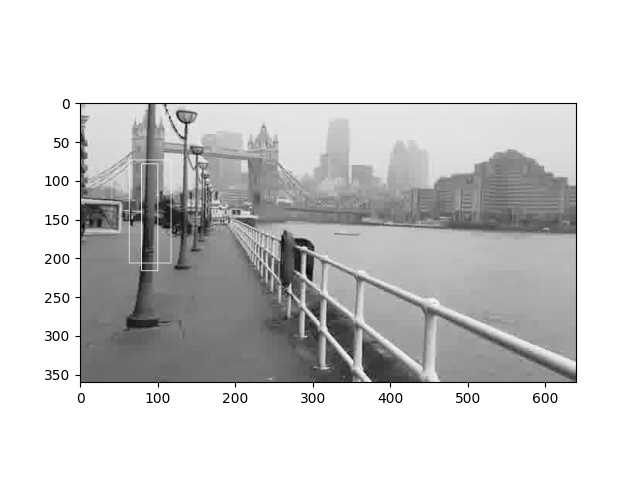
\includegraphics[height=10cm]{vision_50colreg_03.png}

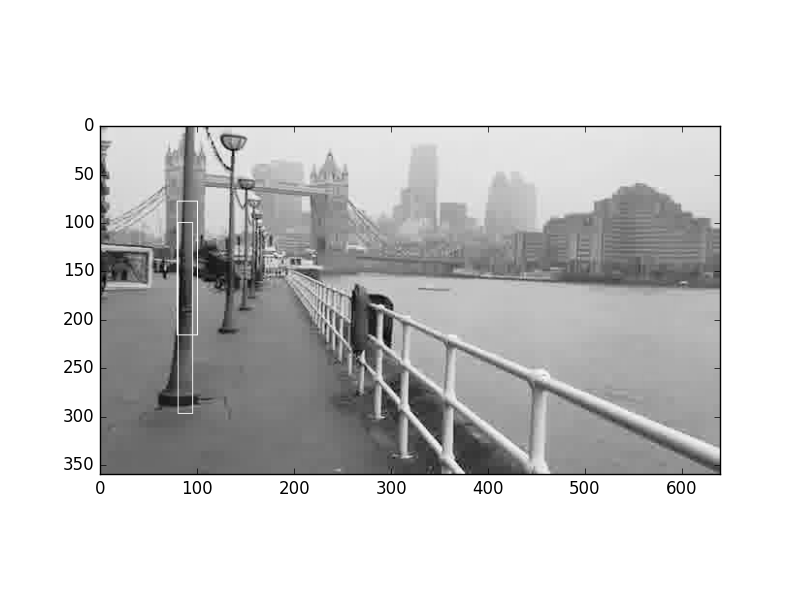
\includegraphics[height=10cm]{vision_50colreg_04.png}

\begin{minted}[fontsize=\footnotesize]{python}
def get_pixels(box, im):
    arr = np.array(im)
    yw = arr.shape[0]
    xw = arr.shape[1]
    (bx1,by1) = box[0]; (bx2,by2) = box[1]
    by1 = yw-by1; by2 = yw-by2
    x1 = min(bx1,bx2); x2 = max(bx1,bx2)
    y1 = min(by1,by2); y2 = max(by1,by2)
    arr = arr[y1:y2, x1:x2]
    return arr
    
im = Image.open('t00100.jpg').convert('L')
arr1 = get_pixels(box1, im) 
arr2 = get_pixels(box2, im) 
print arr1.shape, arr2.shape
\end{minted}

\begin{verbatim}
(138, 21) (133, 54)
\end{verbatim}

Olurluk oranının log'unu alarak hesap yapınca

\begin{minted}[fontsize=\footnotesize]{python}
def likratio(arr1,arr2):
    tarr1 = np.reshape(arr1, (arr1.shape[0]*arr1.shape[1]),1)
    tarr2 = np.reshape(arr2, (arr2.shape[0]*arr2.shape[1]),1)
    arr0 = np.hstack((tarr1,tarr2))
    s0 = np.std(arr0); s1 = np.std(tarr1); s2 = np.std(tarr2)
    L = len(arr0)*np.log(s0) - (len(tarr1)*np.log(s1) + len(tarr2)*np.log(s2))
    return L
L = likratio(arr1, arr2)
print L
\end{minted}

\begin{verbatim}
419.6536187
\end{verbatim}

İkinci resimde her iki dikdörtgen aynı direğin üzerinde, yani aynı obje
üzerindeler. Bu durumda oranın daha düşük olmasını bekleriz,

\begin{minted}[fontsize=\footnotesize]{python}
arr1 = get_pixels(box1, im)
arr2 = get_pixels(box3, im)
L = likratio(arr1, arr2)
print L
\end{minted}

\begin{verbatim}
244.473078548
\end{verbatim}

Hakikaten de öyle.

Çok Boyutlu Gaussian Kullanmak

Eğer renkli resimleri işlemek istiyorsak, her pikselin H,S,V  değerlerini
kullanabiliriz, bu durumda bir resim bölgesini üç boyutlu Gaussian olarak temsil
etmemiz gerekir. Yani üç boyutlu herhangi bir piksel $x_i$ için

$$
p(x_i) =
\frac{1}{(2\pi)^{p/2} \det(\Sigma)^{1/2}} \exp 
\bigg\{  -\frac{1}{2}(x_i-\mu)^T\Sigma^{-1}(x_i-\mu) \bigg\}
$$

$\mu,\Sigma$ bu Gaussian'ın ait olduğu bölge olacaktır, $p$ boyuttur, yani
3. Türetime başlamadan önce $\Sigma$'yi kestirme hesaplayan $\hat{\Sigma}$'yi
hatırlayalım,

$$ \hat{\Sigma} = \frac{1}{n} \sum _{i=1}^{n} (x_i-\hat{\mu}) (x_i-\hat{\mu})^T $$

Kısaltma amaçlı $C_j = 1 / \big((2\pi)^{k/2} \det(\Sigma_j)^{1/2}\big)$ diyelim, 

$$
p(\{x\}|H_0) =
\prod _{i=1}^{m_1+m_2} \frac{1}{C_0}
\exp \bigg[-\frac{ 1}{2}(x_i-\mu_0)^T\Sigma_0^{-1}(x_i-\mu_0) \bigg]
$$

$$ =
\frac{1}{C_0^{m_1+m_2}}
\exp \bigg[\sum _{i=1}^{m_1+m_2} -\frac{ 1}{2}(x_i-\mu_0)^T\Sigma_0^{-1}(x_i-\mu_0) \bigg]
$$

Şimdi aynen tek boyutlu örnekte olduğu gibi $\Sigma_0$ yerine onun kestirme
hesabını formüle sokalım,

$$
= \frac{1}{C_0^{m_1+m_2}} \exp \bigg[\sum _{i=1}^{n} 
-\frac{1}{2}(x_i-\hat{\mu})^T 
\bigg[
\frac{1}{m_1+m_2} \sum _{k=1}^{m_1+m_2} (x_k-\hat{\mu}_0) (x_k-\hat{\mu}_0)^T
\bigg]^{-1}
(x_i-\hat{\mu}_0) \bigg]
$$

Bu formül nasıl kısalabilir? Herhangi bir $\mu$ için $z_i=x_i-\hat{\mu}$
diyelim, $m_1+m_2$ yerine $n$ olsun, ve $z_i$ ifadesi $p \times 1$ boyutunda
vektörler. Genel olarak şu ifadeyi

$$ \sum_{i=1}^n z_i^T\left(\sum_{k=1}^n z_kz_k^T\right)^{-1}z_i $$

kısaltmaya uğraşıyoruz. Burada iz operatörünü kullanabiliriz, iz bildiğimiz gibi
bir matrisin köşegeninin toplamını verir. Güzel özellikleri vardır, mesela
$\tr(A+B)=\tr(A)+\tr(B)$ ve $\tr(AB)=\tr(BA)$ gibi.

$$
\sum_{i=1}^n z_i^T\left(\sum_{k=1}^n z_kz_k^T\right)^{-1}z_i  =
\tr\left[\sum_{i=1}^n z_i^T\left(\sum_{k=1}^n
  z_kz_k^T\right)^{-1}z_i\right] 
$$

ile başlayabiliriz. İz kullanabildik çünkü izini aldığımız ``matris'' aslında
bir tek sayı. Şimdi izin üstteki ve toplam işlemleri içine nüfuz edebilme
özelliğini kullanacağız,

$$= \sum_{i=1}^n\tr\left[ z_i^T\left(\sum_{k=1}^n z_kz_k^T\right)^{-1}z_i\right]$$

$$ = \sum_{i=1}^n\tr\left[ \left(\sum_{k=1}^n z_kz_k^T\right)^{-1}z_iz_i^T\right] $$

$$
= \tr\left[ \left(\sum_{k=1}^n z_kz_k^T\right)^{-1}
\sum_{i=1}^nz_iz_i^T\right] = \tr(I_p)=p 
$$

O zaman 

$$
\exp\left[-\frac12\sum_{i=1}^n z_i^T\left(\frac1n\sum_{k=1}^n
 z_kz_k^T\right)^{-1}z_i\right]  =
\exp\left[-\frac{n}2\sum_{i=1}^n
z_i^T\left(\sum_{k=1}^n z_kz_k^T\right)^{-1}z_i\right]=\exp(-np/2)
$$

haline geldi, demek ki

$$ p(\{x\}|H_0) = \frac{1}{C_0^{m_1+m_2}}\exp\bigg[-\frac{(m_1+m_2)p}{2}\bigg] $$

$$ p(\{x\}|H_1) =
\frac{1}{C_1^{m_1}}\exp\bigg[-\frac{m_1 p}{2}\bigg]
\frac{1}{C_2^{m_2}}\exp\bigg[-\frac{m_2 p}{2}\bigg]
$$

$$ =
\frac{1}{C_1^{m_1}}\frac{1}{C_2^{m_2}}
\exp\bigg[-\frac{m_1 p}{2} -\frac{m_2 p}{2}\bigg]
$$

$$ =
\frac{1}{C_1^{m_1}}\frac{1}{C_2^{m_2}} \exp\bigg[- \frac{(m_1+m_2) p}{2}\bigg]
$$

$$ L = \frac{p(\{x\}|H_1)}{p(\{x\}|H_0)} $$

Bölüm sırasında $\exp$ terimleri iptal olur, sonuç

$$ L = \frac{C_0^{m_1+m_2}}{C_1^{m_1}C_2^{m_2}  } $$

$1/C_j = (2\pi)^{p/2} \det(\Sigma_j)^{1/2} $ oldugu icin

$$
\frac{
  (2\pi)^{m_1 p/2} \det(\Sigma_1)^{m_1/2}
  (2\pi)^{m_2 p/2} \det(\Sigma_2)^{m_2/2}
}
{(2\pi)^{(m_1+m_2) p/2} \det(\Sigma_0)^{(m_1+m_2)/2} }
$$

$$= \frac { |\Sigma_1|^{m_1/2}  |\Sigma_2|^{m_2/2} }{ |\Sigma_0|^{(m_1+m_2)/2} }$$

Tabii hesaptan önce üstteki formülde yine kestirme değerleri yerine koyarak
hesabı yapacağız.

Renkli bir resme bakalım şimdi,

\begin{minted}[fontsize=\footnotesize]{python}
im = Image.open('t00100.jpg').convert('HSV')
print np.array(im).shape
\end{minted}

\begin{verbatim}
(360, 640, 3)
\end{verbatim}

Görüldüğü gibi imaj matrisinde artık her hücrede üç öğe var.

\begin{minted}[fontsize=\footnotesize]{python}
from PIL import Image, ImageDraw
import pandas as pd
import scipy.linalg as lin

def get_pixels(box, arr):
    (yw,xw,d) = arr.shape
    (bx1,by1) = box[0]; (bx2,by2) = box[1]
    by1 = yw-by1; by2 = yw-by2
    x1 = min(bx1,bx2); x2 = max(bx1,bx2)
    y1 = min(by1,by2); y2 = max(by1,by2)
    arr = arr[y1:y2, x1:x2, :]
    return arr

def draw_boxes_color(bs, im):
    arr = np.asarray(im)
    draw = ImageDraw.Draw(im)
    colors = ['magenta','green','white','red','yellow']
    for i,b in enumerate(bs):
        fr = b[0]; to = b[1]
        bnew = [(fr[0],arr.shape[0]-fr[1]),(to[0],arr.shape[0]-to[1])]
        draw.rectangle(bnew,outline=colors[i])
    plt.imshow(im)
    
def loglikratio(box1,box2,arr):
    arr1 = get_pixels(box1, arr)
    arr2 = get_pixels(box2, arr)
    tarr1 = np.reshape(arr1, (arr1.shape[0]*arr1.shape[1],3))
    tarr2 = np.reshape(arr2, (arr2.shape[0]*arr2.shape[1],3))
    tarr0 = np.vstack((tarr1,tarr2))
    sd0 = lin.det(np.cov(tarr0.T))
    sd1 = lin.det(np.cov(tarr1.T))
    sd2 = lin.det(np.cov(tarr2.T))
    LLR = len(tarr0)/2*np.log(sd0) - len(tarr1)/2*np.log(sd1) - len(tarr2)/2*np.log(sd2)
    return LLR
\end{minted}

\begin{minted}[fontsize=\footnotesize]{python}
box1 = [(79,144),(100,282)]
box2 = [(63,154),(117,287)]
box3 = [(80,63),(95,260)]

im = Image.open('t00100.jpg').convert('HSV')
draw_boxes_color([box1,box2],im)
plt.savefig('vision_50colreg_09.png')
im = Image.open('t00100.jpg').convert('HSV')
draw_boxes_color([box1,box3],im)
plt.savefig('vision_50colreg_11.png')
\end{minted}

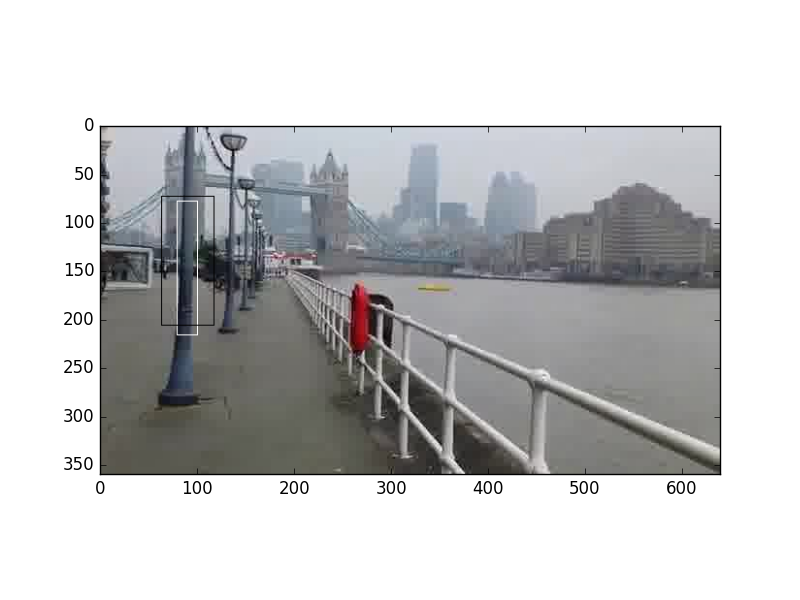
\includegraphics[height=10cm]{vision_50colreg_09.png}

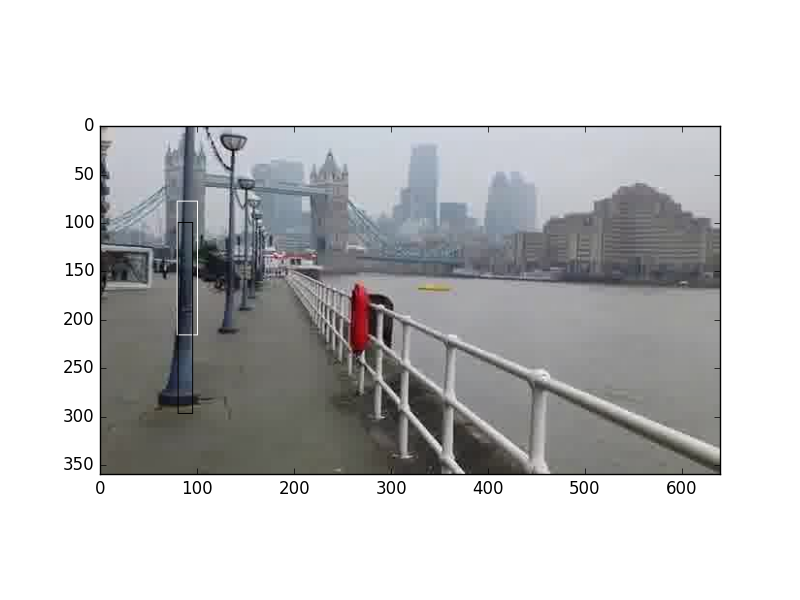
\includegraphics[height=10cm]{vision_50colreg_11.png}

1. ve 2., sonra 1. ve 3. bölgeler arasında olurluk oranını hesaplayalım,

\begin{minted}[fontsize=\footnotesize]{python}
arr = np.array(im)
print  loglikratio(box1,box2,arr) 
print  loglikratio(box1,box3,arr) 
\end{minted}

\begin{verbatim}
874.532775212
635.48295072
\end{verbatim}

Farklı bir resme bakalım, Alcatraz adasının bir fotoğrafı mesela,

\begin{minted}[fontsize=\footnotesize]{python}
box1 = [(36,134),(86,201)]
box2 = [(3,125),(37,200)]
im = Image.open('../vision_01/alcatraz1.png').convert('HSV')
draw_boxes_color([box1,box2],im)
plt.savefig('vision_50colreg_05.png')
\end{minted}

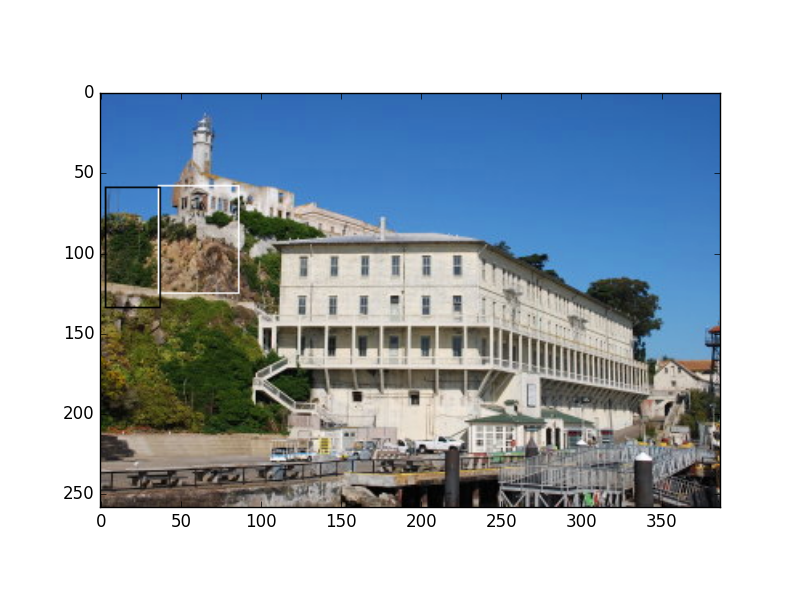
\includegraphics[height=10cm]{vision_50colreg_05.png}

\begin{minted}[fontsize=\footnotesize]{python}
print loglikratio(box1,box2, arr)
\end{minted}

\begin{verbatim}
6599.1051811
\end{verbatim}

\begin{minted}[fontsize=\footnotesize]{python}
box3 = [(19,89),(76,124)]
im = Image.open('../vision_01/alcatraz1.png').convert('HSV')
draw_boxes_color([box1,box3],im)
plt.savefig('vision_50colreg_06.png')
\end{minted}

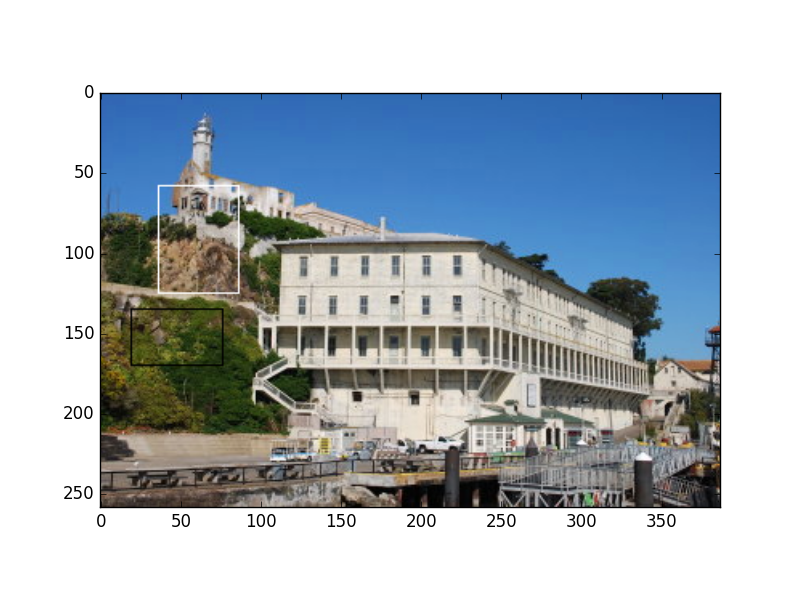
\includegraphics[height=10cm]{vision_50colreg_06.png}

\begin{minted}[fontsize=\footnotesize]{python}
print loglikratio(box1,box3,arr)
\end{minted}

\begin{verbatim}
3171.54541435
\end{verbatim}

Daha zor bir örnek

\begin{minted}[fontsize=\footnotesize]{python}
box1 = [(35,144),(87,292)]
box2 = [(106,183),(158,287)]
box3 = [(117,86),(132,160)]
box4 = [(106,183),(138,287)]
im = Image.open('castle.png').convert('HSV')
draw_boxes_color([box1,box2],im)
plt.savefig('vision_50colreg_07.png')
im = Image.open('castle.png').convert('HSV')
draw_boxes_color([box2,box3],im)
plt.savefig('vision_50colreg_08.png')
im = Image.open('castle.png').convert('HSV')
draw_boxes_color([box1,box4],im)
plt.savefig('vision_50colreg_10.png')
\end{minted}

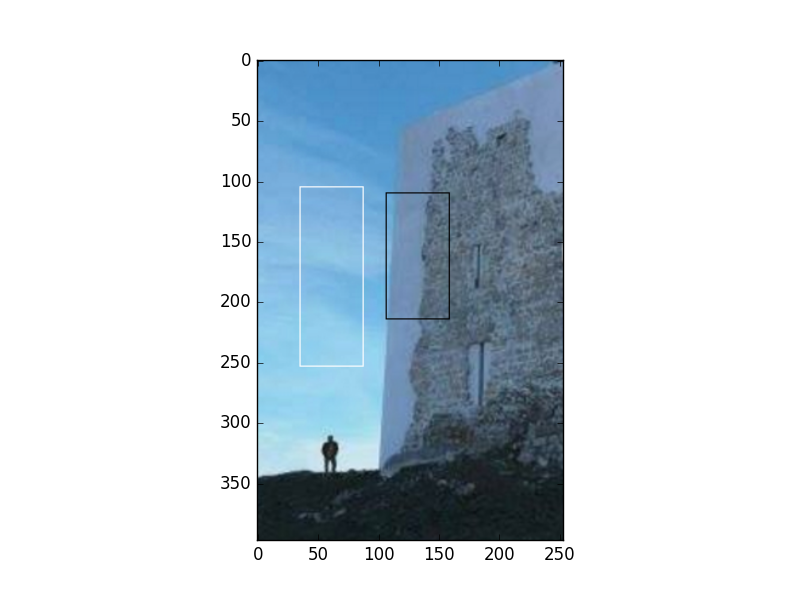
\includegraphics[height=10cm]{vision_50colreg_07.png}

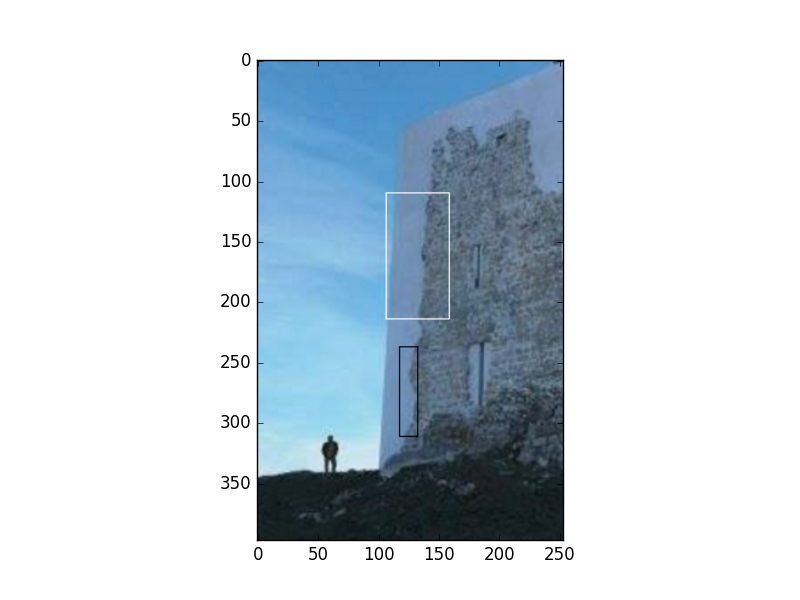
\includegraphics[height=10cm]{vision_50colreg_08.png}

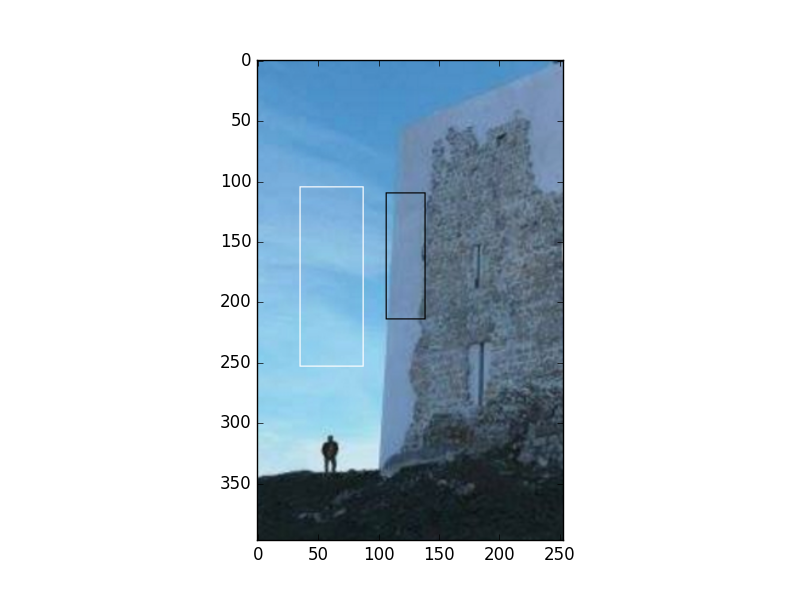
\includegraphics[height=10cm]{vision_50colreg_10.png}

\begin{minted}[fontsize=\footnotesize]{python}
im = Image.open('castle.png').convert('HSV')
arr = np.array(im)
print loglikratio(box1,box2,arr)
print loglikratio(box2,box3,arr)
print loglikratio(box1,box3,arr)
print loglikratio(box1,box4,arr)
\end{minted}

\begin{verbatim}
23886.6334257
527.840460625
15695.3369086
17913.2279323
\end{verbatim}

Kaynaklar

[1] Schunk, {\em Machine Vision}  

[2] Dhakar, {\em Color Thief}, \url{https://github.com/fengsp/color-thief-py}


\end{document}
